\section{Résultats et interprétations}

Nous avons fait tourner cette simulation pour une durée totale physique de 7284 secondes. \FIXME{physique?} 

\subsection{Suivi de la courbe en S}
Les solutions pour chaque $r$ de la branche supérieure déterminées par dichotomie ne sont pas équivalentes aux branches atteintes dans la simulation. Nous pouvons voir sur la figure (\ref{fig:qmap}) en rouge la branche déterminée par dichotomie correspondant à $\tau_\mathrm{ff} = 0.06 $ et en blanc celle correspondant à la valeur théorique $\tau_\mathrm{ff} = 1$. Les possibles raisons de ces écarts sont dévelopés partie (\ref{sec::pistes}). La simulation est bien en accord avec le passage d'un disque optiquement épais à un disque optiquement mince. Nous pouvons voir figure (\ref{fig:c1.eps}) et (\ref{fig:c20.eps}) comment se comporte le système du point de vue de ces deux grandeurs physiques. \FIXME{parler de l'instabilité} \\
 

\begin{figure}
  \begin{center}
    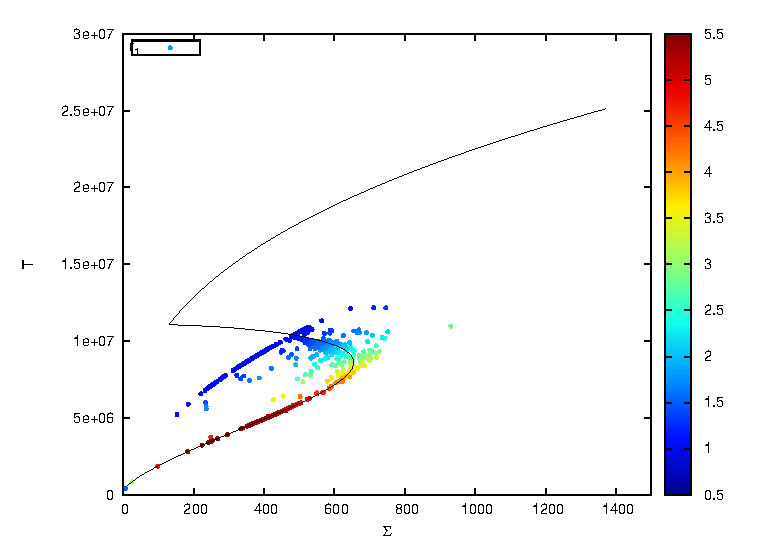
\includegraphics[]{c1.eps}
  \end{center}
  \caption{$T=f(\Sigma)$, $\Delta t = 7284 s$ (durée de la simulation) pour $r_{1}$. Le gradiant de couleur représente les valeurs de $\tau_\mathrm{ff}$}
  \label{fig:c1.eps}
\end{figure} 

\begin{figure}
  \begin{center}
    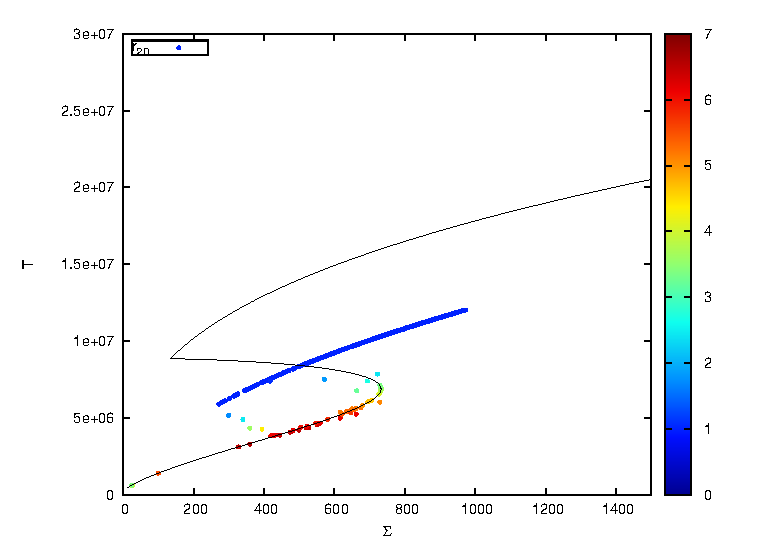
\includegraphics[]{c20.eps}
  \end{center}
  \caption{$T=f(\Sigma)$, $\Delta t = 7284 s$ (durée de la simulation) pour $r_{20}$. Le gradiant de couleur représente les valeurs de $\tau_\mathrm{ff}$}
  \label{fig:c20.eps}
\end{figure}

\subsection{Évolution de la luminosité}

La luminosité a été approximée via $L_\mathrm{tot} = \int_{r_\mathrm{min}}^{r_\mathrm{max}} 2\pi r Fz\ \mathrm{d}r$. Comme attendu, la simulation montre que la luminosité totale du disque n'est pas constante et possède des sursauts, correspondant à l'instabilité. On trouvera en figure \ref{fig:Ltot_function_t} le luminosité simulée au cours du temps pour notre simulation. Dans un premier temps, qui correspond à l'ajout de plus en plus important de matière ($\dot{M}_0$ croissant), sa luminosité augmente lentement dans le domaine énergétique de $10^{21}$ à $10^{24}\ \mathrm{erg.s^{1}}$. Lorsque le disque entre dans l'instabilité, la luminosité croît fortement pour atteindre $10^{25}$ à $10^{27}\ \mathrm{erg.s^{-1}}$. Un détail de la luminosité sur une instabilité est donné sur la figure \ref{fig:Ltot_instabilite}. La non-régularité de la luminosité (sa déviation standard est de l'ordre de grandeur de sa moyenne) laissent à penser que la simulation numérique ne résoud pas correctement l'instabilité. En revanche, on constate que la luminosité moyenne durant l'instabilité est $7.6\ 10^{25}\mathrm{erg.s^{-1}}$, valeur qui est un ordre de grandeur plus important que la luminosité dans le régime stable.
\begin{figure}
  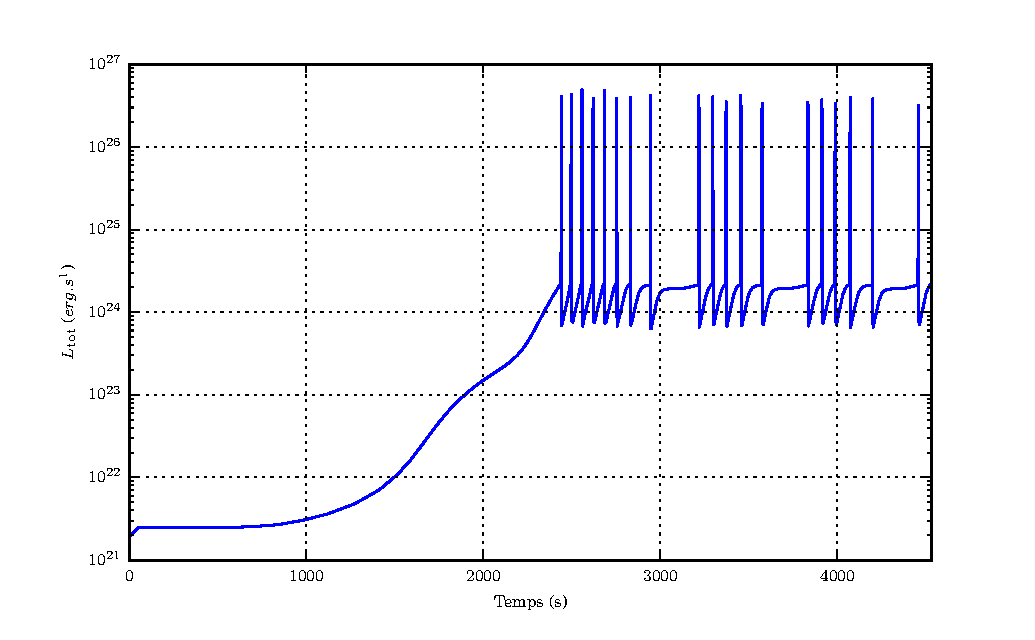
\includegraphics{figures/Ltot_fonction_t.pdf}
  \caption{Simulation de la luminosité $L_\mathrm{tot}$ au cours du temps. L'instabilité se déclenche à $t \approx 2300s$ et se répète régulièrement.}
  \label{fig:Ltot_function_t}
\end{figure}

\begin{figure}
  
  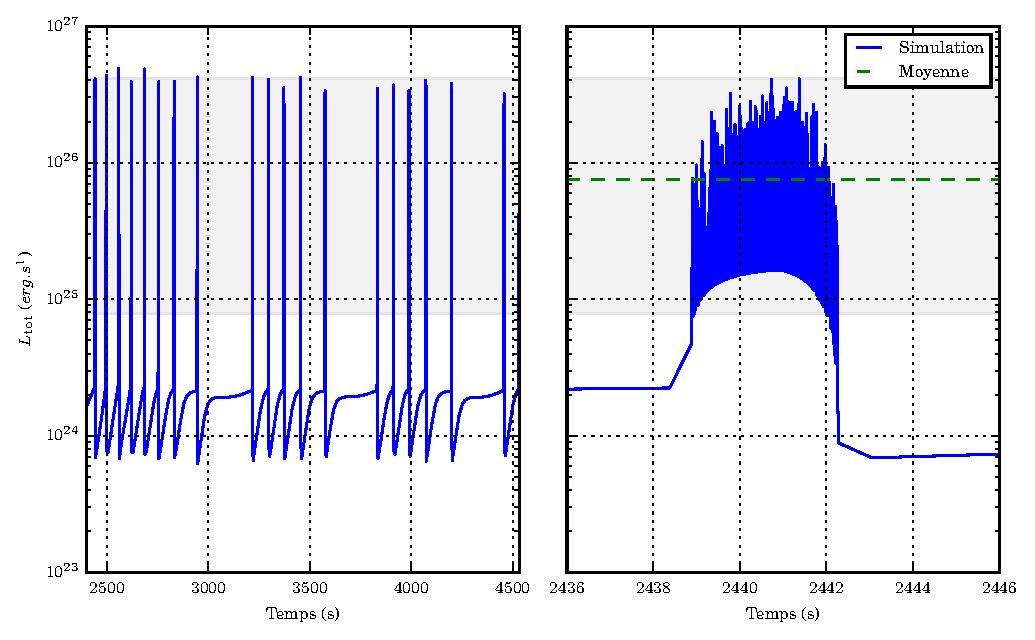
\includegraphics{figures/Ltot_fonction_t_doublecheeseburger.pdf}
  \caption{Simulation de la luminosité $L_\mathrm{tot}$ lors de l'instabilité. À gauche, un dizaine d'instabilités sont observées. À droite, un zoom sur la première instabilité. Sa moyenne est tracée en verte. L'applat gris est délimité par le maximum et le minimum de luminosité sur l'instabilité. On notera par ailleurs que la déviation standard de la luminosité y est du même ordre de grandeur que sa moyenne.}
  \label{fig:Ltot_instabilite}
\end{figure}
%%% Local Variables:
%%% mode: latex
%%% TeX-master: "rapport"
%%% End:
